\documentclass[a4paper, 12pt]{article}

\usepackage{etoolbox}
\makeatletter
\patchcmd\l@section{%
  \nobreak\hfil\nobreak
}{%
  \nobreak
  \leaders\hbox{%
    $\m@th \mkern \@dotsep mu\hbox{.}\mkern \@dotsep mu$%
  }%
  \hfill
  \nobreak
}{}{\errmessage{\noexpand\l@section could not be patched}}
\makeatother

\setcounter{secnumdepth}{0}

\usepackage{float}
\usepackage{graphicx}
\usepackage{caption}
\usepackage{subcaption}
\usepackage{enumitem}
\usepackage{booktabs}
\usepackage[portuges]{babel}
\usepackage[utf8x]{inputenc}
\usepackage{comment}
\usepackage{fullpage}
\usepackage{xcolor}
\usepackage{amsmath,amsfonts,amssymb,amsthm, bm}
\usepackage{csvsimple}
\usepackage{booktabs}
\usepackage{longtable}

\usepackage{listings}
\usepackage{color}
\usepackage{tikz}
\usetikzlibrary{positioning,decorations.pathreplacing}
\usepackage{hyperref}


\definecolor{mygreen}{RGB}{28,172,0}
\definecolor{mylilas}{RGB}{170,55,241}
\renewcommand{\min}{\expandafter\,\operatorname*{min}}

% Default fixed font does not support bold face
\DeclareFixedFont{\ttb}{T1}{txtt}{bx}{n}{12} % for bold
\DeclareFixedFont{\ttm}{T1}{txtt}{m}{n}{12}  % for normal

% Custom colors
\usepackage{color}
\definecolor{deepblue}{rgb}{0,0,0.5}
\definecolor{deepred}{rgb}{0.6,0,0}
\definecolor{deepgreen}{rgb}{0,0.5,0}

\usepackage{listings}

% Python style for highlighting
\newcommand\pythonstyle{\lstset{
language=Python,
basicstyle=\ttm,
otherkeywords={self},             % Add keywords here
keywordstyle=\ttb\color{deepblue},
emph={MyClass,__init__},          % Custom highlighting
emphstyle=\ttb\color{deepred},    % Custom highlighting style
stringstyle=\color{deepgreen},
frame=tb,                         % Any extra options here
showstringspaces=false            % 
}}


% Python environment
\lstnewenvironment{python}[1][]
{
\pythonstyle
\lstset{#1}
}
{}

% Python for external files
\newcommand\pythonexternal[2][]{{
\pythonstyle
\lstinputlisting[#1]{#2}}}

% Python for inline
\newcommand\pythoninline[1]{{\pythonstyle\lstinline!#1!}}


\begin{document}
\noindent
\large\textbf{Lista de Exercícios 3} \hfill \textbf{Luis Vinicius Costa Silva} \\
\normalsize Otimização Clássica \\
Prof. Romes Antonio Borges \\
\hfill Data de Entrega: 10/06/2019
\tableofcontents

\section*{Questão 1}
\subsection*{Item A}
Considerando o problema de otimização abaixo:


\begin{align*}
\begin{split}
\text{min\phantom{0}} f(x) = (x_1 - 1)^2 + (x_2 - 1)^2 \text{\phantom{000} s.t:} \\
x_1 + x_2 -1 \leq 0	 \\
x_1 \leq 0
\end{split}
\end{align*}

Este problema de otimização foi resolvido utilizando o Método da Penalidade Exterior através do Método de Nelder-Mead. Para tanto, o problema foi reescrito como um problema de otimização irrestrita usando uma função pseudo-objetivo da seguinte forma:

\begin{align*}
\begin{split}
\text{min\phantom{0}} f'(x) = F(x) + r_p P(x) \text{\phantom{000} tal que P(x) é dado por:} \\
P(x) = \sum_{i=1}^{n} (max(0,g_i(x)))^2 + \sum_{j=1}^{m} (h_k(x))^2 \\
f'(x) = (x_1-1)^2 + (x_2-1)^2 + r_p max (0,x_1+x_2-1)^2
\end{split}
\end{align*}


Foi encontrado como $x^*$ o ponto $(\frac{1}{2},\frac{1}{2},\frac{1}{2})$ A figuras \ref{fig:Q1ARP1}, \ref{fig:Q1ARP10}, \ref{fig:Q1ARP100} e \ref{fig:Q1ARP1000} apresentam as curvas de nível e as superfície da função para cada $r_p$, assim como a convergência do algoritmo em cada execução:

\begin{figure}[H]
\centering
\begin{subfigure}{0.3\textwidth}
  \centering
  \includegraphics[width=\linewidth]{1/A/RP1/contorno.png}
  %\caption{A subfigure}
\end{subfigure}%
\begin{subfigure}{0.3\textwidth}
  \centering
  \includegraphics[width=\linewidth]{1/A/RP1/superficie.png}
  %\caption{A subfigure}
\end{subfigure}
\begin{subfigure}{0.3\textwidth}
  \centering
  \includegraphics[width=\linewidth]{1/A/RP1/convergencia.png}
  %\caption{A subfigure}
\end{subfigure}
\caption{Curvas de nível, superfícies e séries de convergência para $r_p = 1$}
\label{fig:Q1ARP1}
\end{figure}

\begin{figure}[H]
\centering
\begin{subfigure}{0.3\textwidth}
  \centering
  \includegraphics[width=\linewidth]{1/A/RP10/contorno.png}
  %\caption{A subfigure}
\end{subfigure}%
\begin{subfigure}{0.3\textwidth}
  \centering
  \includegraphics[width=\linewidth]{1/A/RP10/superficie.png}
  %\caption{A subfigure}
\end{subfigure}
\begin{subfigure}{0.3\textwidth}
  \centering
  \includegraphics[width=\linewidth]{1/A/RP10/convergencia.png}
  %\caption{A subfigure}
\end{subfigure}
\caption{Curvas de nível, superfícies e séries de convergência para $r_p = 10$}
\label{fig:Q1ARP10}
\end{figure}

\begin{figure}[H]
\centering
\begin{subfigure}{0.3\textwidth}
  \centering
  \includegraphics[width=\linewidth]{1/A/RP1/contorno.png}
  %\caption{A subfigure}
\end{subfigure}%
\begin{subfigure}{0.3\textwidth}
  \centering
  \includegraphics[width=\linewidth]{1/A/RP1/superficie.png}
  %\caption{A subfigure}
\end{subfigure}
\begin{subfigure}{0.3\textwidth}
  \centering
  \includegraphics[width=\linewidth]{1/A/RP1/convergencia.png}
  %\caption{A subfigure}
\end{subfigure}
\caption{Curvas de nível, superfícies e séries de convergência para $r_p = 100$}
\label{fig:Q1ARP100}
\end{figure}

\begin{figure}[H]
\centering
\begin{subfigure}{0.3\textwidth}
  \centering
  \includegraphics[width=\linewidth]{1/A/RP1/contorno.png}
  %\caption{A subfigure}
\end{subfigure}%
\begin{subfigure}{0.3\textwidth}
  \centering
  \includegraphics[width=\linewidth]{1/A/RP1/superficie.png}
  %\caption{A subfigure}
\end{subfigure}
\begin{subfigure}{0.3\textwidth}
  \centering
  \includegraphics[width=\linewidth]{1/A/RP1/convergencia.png}
  %\caption{A subfigure}
\end{subfigure}
\caption{Curvas de nível, superfícies e séries de convergência para $r_p = 1000$}
\label{fig:Q1ARP1000}
\end{figure}

As tabelas abaixo geraram os dados apresentados acima:

% Please add the following required packages to your document preamble:
% \usepackage{longtable}
% Note: It may be necessary to compile the document several times to get a multi-page table to line up properly
\begin{longtable}[c]{|l|l|l|l|}
\hline
\multicolumn{1}{|c|}{x\_1} & \multicolumn{1}{c|}{x\_2} & \multicolumn{1}{c|}{f(x)} & \multicolumn{1}{c|}{erro} \\ \hline
\endfirsthead
%
\multicolumn{4}{c}%
{{\bfseries Continuação da Tabela \thetable\ da página anterior}} \\
\hline
\multicolumn{1}{|c|}{x\_1} & \multicolumn{1}{c|}{x\_2} & \multicolumn{1}{c|}{f(x)} & \multicolumn{1}{c|}{erro} \\ \hline
\endhead
%
0.6666666850283716         & 0.6666669105274989        & 0.22222204740725726       & 0.6466666666665379        \\ \hline
0.5714287679821353         & 0.5714283239884842        & 0.3673469823926301        & 0.1269844766143351        \\ \hline
0.526315496942255          & 0.5263160380993406        & 0.4487535041989682        & 0.07733611040286753       \\ \hline
0.5090905298560064         & 0.5090912957665924        & 0.4819834637691798        & 0.03263653227211932       \\ \hline
0.5030672383633491         & 0.5030676827213969        & 0.49388389754371076       & 0.011827829852086247      \\ \hline
0.5010262308757442         & 0.5010271600635555        & 0.4979487172683068        & 0.0040564449704547645     \\ \hline
0.5003425150025591         & 0.5003429195586395        & 0.49931480034915204       & 0.0013651838080389611     \\ \hline
0.5001138951133319         & 0.5001146850146494        & 0.4997714459967681        & 0.0004565835788785666     \\ \hline
0.5000379759302219         & 0.5000382154495984        & 0.49992381152277154       & 0.00015235190822671107    \\ \hline
0.5000131528815173         & 0.5000122494888153        & 0.4999745979527157        & 5.0774817701215724e-05    \\ \hline
0.5000045189438189         & 0.50000394786201          & 0.4999915332301776        & 1.6934852061833983e-05    \\ \hline
0.500031101335553          & 0.4999716884127744        & 0.4999972120205117        & 5.641630192065872e-06     \\ \hline
0.5000382193108293         & 0.49996266826569685       & 0.49999911527784807       & 1.814121249499312e-06     \\ \hline
0.5000403144241239         & 0.49995998863623353       & 0.49999970016580453       & 5.246755701571182e-07     \\ \hline
\caption{Para $r_P = 1$}
\label{tab:Q1ARP1}\\
\end{longtable}

% Please add the following required packages to your document preamble:
% \usepackage{longtable}
% Note: It may be necessary to compile the document several times to get a multi-page table to line up properly
\begin{longtable}[c]{|l|l|l|l|}
\hline
x\_1                & x\_2               & f(x)                & erro                   \\ \hline
\endfirsthead
%
\multicolumn{4}{c}%
{{\bfseries Continuação da Tabela \thetable\ da página anterior}} \\
\hline
x\_1                & x\_2               & f(x)                & erro                   \\ \hline
\endhead
%
0.5238096685439415  & 0.523809244532719  & 0.45351486736473057 & 0.5038095238092439     \\ \hline
0.5081970921637178  & 0.5081964963344485 & 0.4837407863739348  & 0.029738415153455655   \\ \hline
0.5027626309141939  & 0.5027621944048724 & 0.49449043652843205 & 0.010690694259194      \\ \hline
0.5009245672444872  & 0.5009238660283281 & 0.4981532750802126  & 0.0036560485435986334  \\ \hline
0.5003088837966202  & 0.5003080364167611 & 0.49938327008225253 & 0.0012292581596012875  \\ \hline
0.5001026581896479  & 0.5001030559664557 & 0.49979430700313254 & 0.00041096461176692856 \\ \hline
0.5000343457642397  & 0.5000342296817712 & 0.49993142690529174 & 0.00013709871286693431 \\ \hline
0.5000115590903891  & 0.5000113038103384 & 0.4999771373606612  & 4.5703510737515884e-05 \\ \hline
0.5000036285854446  & 0.5000039936094471 & 0.49999237783422384 & 1.5242875561982672e-05 \\ \hline
0.49997368156102384 & 0.5000288401868227 & 0.49999747977657005 & 5.08177470931459e-06   \\ \hline
0.49996535376827844 & 0.5000354251072681 & 0.4999992235797531  & 1.6530289737026749e-06 \\ \hline
0.4999631727298208  & 0.5000371349670335 & 0.49999969503839925 & 4.3548042966135014e-07 \\ \hline
\caption{Para $r_P = 10$}
\label{tab:Q1ARP10}\\
\end{longtable}


% Please add the following required packages to your document preamble:
% \usepackage{longtable}
% Note: It may be necessary to compile the document several times to get a multi-page table to line up properly
\begin{longtable}[c]{|l|l|l|l|}
\hline
x\_1               & x\_2                & f(x)                & erro                   \\ \hline
\endfirsthead
%
\multicolumn{4}{c}%
{{\bfseries Continuação da Tabela \thetable\ da página anterior}} \\
\hline
x\_1               & x\_2                & f(x)                & erro                   \\ \hline
\endhead
%
0.5024871168079972 & 0.5024880076082603  & 0.49503725151561795 & 0.4824875621886578     \\ \hline
0.5008323270357756 & 0.5008315439308794  & 0.4983375132669485  & 0.0032947571577385815  \\ \hline
0.5002772463765501 & 0.5002780072735618  & 0.49944490050348556 & 0.001106756743406212   \\ \hline
0.5000929320720773 & 0.5000922321579115  & 0.49981485291315214 & 0.00036990381485046964 \\ \hline
0.5000307611547639 & 0.5000309724391769  & 0.4999382683115998  & 0.00012343012066895476 \\ \hline
0.5000101543791571 & 0.5000104228200435  & 0.49997942301254605 & 4.1164355555678434e-05 \\ \hline
0.5000035161825714 & 0.5000033415514702  & 0.4999931422894879  & 1.3719744382245658e-05 \\ \hline
0.5000266233333861 & 0.4999756263262689  & 0.4999977516432228  & 4.5689489297506825e-06 \\ \hline
0.5000317671950696 & 0.49996899670474415 & 0.49999923807054525 & 1.4512116387477292e-06 \\ \hline
0.5000333806920074 & 0.49996693183161817 & 0.49999968968414876 & 5.047280742798144e-07  \\ \hline
\caption{Para $r_P = 100$}
\label{tab:Q1ARP100}\\
\end{longtable}

% Please add the following required packages to your document preamble:
% \usepackage{longtable}
% Note: It may be necessary to compile the document several times to get a multi-page table to line up properly
\begin{longtable}[c]{|l|l|l|l|}
\hline
x\_1                & x\_2               & f(x)                & erro                   \\ \hline
\endfirsthead
%
\multicolumn{4}{c}%
{{\bfseries Continuação da Tabela \thetable\ da página anterior}} \\
\hline
x\_1                & x\_2               & f(x)                & erro                   \\ \hline
\endhead
%
0.5002501733302913  & 0.5002495894221257 & 0.4995003621291578  & 0.4802498750621386     \\ \hline
0.5000833337151517  & 0.5000832907545782 & 0.49983338941212796 & 0.00033297000140197763 \\ \hline
0.5000276692410743  & 0.5000278776439161 & 0.4999444546577595  & 0.00011103907169396354 \\ \hline
0.5000095943242626  & 0.5000089265354448 & 0.49998147931202663 & 3.702106880415501e-05  \\ \hline
0.500002612743998   & 0.5000035619948071 & 0.49999382528070907 & 1.2350513761860693e-05 \\ \hline
0.49998803955029925 & 0.5000140164105236 & 0.4999979443786893  & 4.118705150601976e-06  \\ \hline
0.4999812879363457  & 0.5000193244662279 & 0.49999938832100277 & 1.3641204836822851e-06 \\ \hline
0.499979664177176   & 0.5000205906985109 & 0.49999974596183566 & 3.204938402445734e-07  \\ \hline
\caption{Para $r_P = 1000$}
\label{tab:Q1ARP1000}\\
\end{longtable}

\subsection*{Item B}
A obtenção do $\Phi$ ótimo e os valores e os valores associados de $x_1$, $x_2$, $g_1$ e $g_2$ para $r_P = 1.0$ e $r_P = 10$ foi feita da seguinte forma:

\begin{align*}
\begin{split}
\phi(x) = F(x) + r_P * \sum_{i=1}^{m} (max(0,g_i(x)))^2 + \sum_{j=1}^{n} (h_j(x))^2 \\
\phi(x) = (x_1 - 1)^2 + (x_2 - 1)^2 + r_p max(0,x_1+x_2-1)^2
\end{split}
\end{align*}

Para $\nabla \phi(x) = 0$ temos que:

\begin{align*}
\begin{split}
\left\{\begin{matrix}
2(x_1 - 1) + 2 r_P (x_1 + x_2- 1 ) = & 0 \\ 
2(x_2 - 1) + 2 r_P (x_1 + x_2- 1 ) = & 0 \\ 
\end{matrix}\right.
\end{split}
\end{align*}

Logo, $x_1 = x_2 = \frac{2 + 2 r_P}{2 + 4 r_P}$. Assim, para $r_P = 1$, temos que  $(x_1,x_2,\phi, g_1, g_2)^* = (\frac{4}{6}, \frac{4}{6}, \frac{1}{3}, \frac{1}{3}, \frac{2}{3})$ e de forma análoga, para $r_P = 10$ temos que \newline
$(x_1,x_2,\phi, g_1, g_2)^* = (\frac{22}{42},\frac{22}{42},0.4762,0.4762,0.5238)$.
\subsection*{Item C}

\subsection*{Item D}
No item D, foi otimizada a função do item A com $r_p = 10$ através do algoritmo de Nelder-Mead utilizando o Método da Penalidade da função exterior. Foi variado o chute inicial para cada execução, tais que os testes foram feitos para $x_0 = (1.0, 1.0)$, $x_0 = {10.0, 10.0}$ e $x_0 = {-1.0, 1.0}$.
A figuras \ref{fig:x1x1}, \ref{fig:x10x10} e \ref{fig:x-1x1} apresentam as curvas de nível e as superfície da função para cada $x_0$, assim como a convergência do algoritmo em cada execução:

\begin{figure}[H]
\centering
\begin{subfigure}{0.3\textwidth}
  \centering
  \includegraphics[width=\linewidth]{1/D/x1x1/contorno.png}
  %\caption{A subfigure}
\end{subfigure}%
\begin{subfigure}{0.3\textwidth}
  \centering
  \includegraphics[width=\linewidth]{1/D/x1x1/superficie.png}
  %\caption{A subfigure}
\end{subfigure}
\begin{subfigure}{0.3\textwidth}
  \centering
  \includegraphics[width=\linewidth]{1/D/x1x1/convergencia.png}
  %\caption{A subfigure}
\end{subfigure}
\caption{Curvas de nível, superfícies e séries de convergência para $x = (1.0, 1.0)$}
\label{fig:x1x1}
\end{figure}

\begin{figure}[H]
\centering
\begin{subfigure}{0.3\textwidth}
  \centering
  \includegraphics[width=\linewidth]{1/D/x10x10/contorno.png}
  %\caption{A subfigure}
\end{subfigure}%
\begin{subfigure}{0.3\textwidth}
  \centering
  \includegraphics[width=\linewidth]{1/D/x10x10/superficie.png}
  %\caption{A subfigure}
\end{subfigure}
\begin{subfigure}{0.3\textwidth}
  \centering
  \includegraphics[width=\linewidth]{1/D/x10x10/convergencia.png}
  %\caption{A subfigure}
\end{subfigure}
\caption{Curvas de nível, superfícies e séries de convergência para $x = (10.0, 10.0)$}
\label{fig:x10x10}
\end{figure}

\begin{figure}[H]
\centering
\begin{subfigure}{0.3\textwidth}
  \centering
  \includegraphics[width=\linewidth]{1/D/x-1x1/contorno.png}
  %\caption{A subfigure}
\end{subfigure}%
\begin{subfigure}{0.3\textwidth}
  \centering
  \includegraphics[width=\linewidth]{1/D/x-1x1/superficie.png}
  %\caption{A subfigure}
\end{subfigure}
\begin{subfigure}{0.3\textwidth}
  \centering
  \includegraphics[width=\linewidth]{1/D/x-1x1/convergencia.png}
  %\caption{A subfigure}
\end{subfigure}
\caption{Curvas de nível, superfícies e séries de convergência para $x = (-1.0, 1.0)$}
\label{fig:x-1x1}
\end{figure}

Nota-se que o algoritmo de otimização foi capaz de convergir para o ótimo da função com o mesmo número de iterações (13 iterações) e com razões de convergências idênticas, independentemente do chute inicial fornecido. Tal fato demonstra a robustez do método, visto que o seu correto funcionamento não é demasiadamente sensível aos parâmetros de entrada em casos onde a função objetivo e suas restrições são bem comportados (i.e: contínuos, diferenciáveis, etc.).

\subsection*{Item E}
Considerando o problema de otimização do Item A, este foi reformulado para ser reescrito como uma função pseudo-objetivo utilizando o Método da Penalidade Interior, da seguinte forma:


\begin{align*}
\begin{split}
\text{min\phantom{0}} f'(x) = F(x) + r_p P(x) \text{\phantom{000} tal que P(x) é dado por:} \\
P(x) = \sum_{i=1}^{m} (\overline g_i(x)) +  \sum_{j=1}^{n} (h_j(x))^2 \\
\overline g_i(x) = 
\left\{\begin{matrix}
\frac{-1}{g_i(x)} \leftrightarrow g_i(x) \leq  \epsilon  \\ 
\frac{-2 \epsilon - g_i(x)}{\epsilon^2} | \epsilon = -C {r_P}^a, 
\end{matrix}\right.
\end{split}
\end{align*}


Utilizando o método de Nelder-Mead e $r_P = 10.0$ para minimizar a função descrita, obteve-se os seguintes resultado:


\begin{figure}[H]
\centering
\begin{subfigure}{0.3\textwidth}
  \centering
  \includegraphics[width=\linewidth]{1/E/NelderMead/contorno.png}
  %\caption{A subfigure}
\end{subfigure}%
\begin{subfigure}{0.3\textwidth}
  \centering
  \includegraphics[width=\linewidth]{1/E/NelderMead/superficie.png}
  %\caption{A subfigure}
\end{subfigure}
\begin{subfigure}{0.3\textwidth}
  \centering
  \includegraphics[width=\linewidth]{1/E/NelderMead/convergencia.png}
  %\caption{A subfigure}
\end{subfigure}
\caption{Curvas de nível, superfícies e séries de convergência para o item E - Nelder-Mead}
\label{fig:x-1x1}
\end{figure}


\begin{longtable}[c]{|l|l|l|l|}
\hline
x\_1                & x\_2                 & f(x)               & erro                   \\ \hline
\endfirsthead
%
\multicolumn{4}{c}%
{{\bfseries Continuação da Tabela \thetable\ da página anterior}} \\
\hline
x\_1                & x\_2                 & f(x)               & erro                   \\ \hline
\endhead
%
-0.4337297515632955 & -0.43373030102459964 & 4.111163576593839  & 15.89989389334903      \\ \hline
0.2623354976138911  & 0.26233505431145676  & 1.088298490178227  & 2.500092645260892      \\ \hline
0.4497588265423719  & 0.44975943227194093  & 0.6055300313417242 & 0.3955656496019184     \\ \hline
0.49046768009506486 & 0.49046812505764736  & 0.5192459166099743 & 0.0705425236826952     \\ \hline
0.49824650006328    & 0.4982459867333184   & 0.5035136645279694 & 0.012860055488568611   \\ \hline
0.4996794192146522  & 0.49967927179479465  & 0.5006415146291747 & 0.0023477842738919286  \\ \hline
0.49994177847045607 & 0.49994111149546056  & 0.5001171168916858 & 0.00042865470298514285 \\ \hline
0.4999892970271441  & 0.4999893177539732   & 0.5000213854475468 & 7.82544014724662e-05   \\ \hline
0.5000353872566405  & 0.4999606081450917   & 0.5000040074022439 & 1.4284741416514812e-05 \\ \hline
0.5000235378709201  & 0.49997581335974817  & 0.5000006499083567 & 2.7012590907427025e-06 \\ \hline
0.500021676812469   & 0.4999781936359934   & 0.5000001304969393 & 4.147939658416533e-07  \\ \hline
\caption{Resolução via MPFI + Nelder-Mead p/ $r_P = 10.0$}
\label{tab:Q1ENelder-Mead}\\
\end{longtable}

\section*{Questão 2}
\subsection*{Item A}

Dado o problema de otimização abaixo:

\begin{align*}
\begin{split}
\text{min\phantom{0}} f(x) = (x_1 - 1)^2 + (x_2 - 1)^2 \text{\phantom{000} s.t:} \\
x_1 - x_2 - 2 = 0
\end{split}
\end{align*}

Reescrevendo o problema de otimização acima utilizando uma função pseudo-objetiva da forma de Lagrangeano Aumentado, temos:
\begin{align*}
\begin{split}
A(x, \lambda, r_P) = F(x) + \sum_{i=1}^{l} (\lambda_i h_i(x) + r_P (h_i(x))^2) \\
A(x, \lambda, r_P) = (x_1 - 1)^2 + (x_2 - 1)^2 + \lambda (x_1 - x_2 - 2) + r_P (x_1 - x_2 - 2)^2
\end{split}
\end{align*}

Reescrevendo o problema de otimização acima utilizando uma função pseudo-objetiva da forma de Penalidade Interior, temos:

\begin{align*}
\begin{split}
\text{min\phantom{0}} f'(x) = F(x) + r_p P(x) \text{\phantom{000} tal que P(x) é dado por:} \\
P(x) = \sum_{i=1}^{m} (\overline g_i(x)) +  \sum_{j=1}^{n} (h_j(x))^2 \\
\overline g_i(x) = 
\left\{\begin{matrix}
\frac{-1}{g_i(x)} \leftrightarrow g_i(x) \leq  \epsilon  \\ 
\frac{-2 \epsilon - g_i(x)}{\epsilon^2} | \epsilon = -C {r_P}^a, 
\end{matrix}\right. \\
f'(x) = (x_1-1)^2 + (x_2-1)^2 + (x_1+x_2-2)^2
\end{split}
\end{align*}

Na forma de Penalidade Exterior, temos:
\begin{align*}
\begin{split}
\text{min\phantom{0}} f'(x) = F(x) + r_p P(x) \text{\phantom{000} tal que P(x) é dado por:} \\
P(x) = \sum_{i=1}^{n} (max(0,g_i(x)))^2 + \sum_{j=1}^{m} (h_k(x))^2 \\
f'(x) = (x_1-1)^2 + (x_2-1)^2 + (x_1+x_2-2)^2
\end{split}
\end{align*}
\subsection{Item B}



\begin{figure}[H]
  \centering
  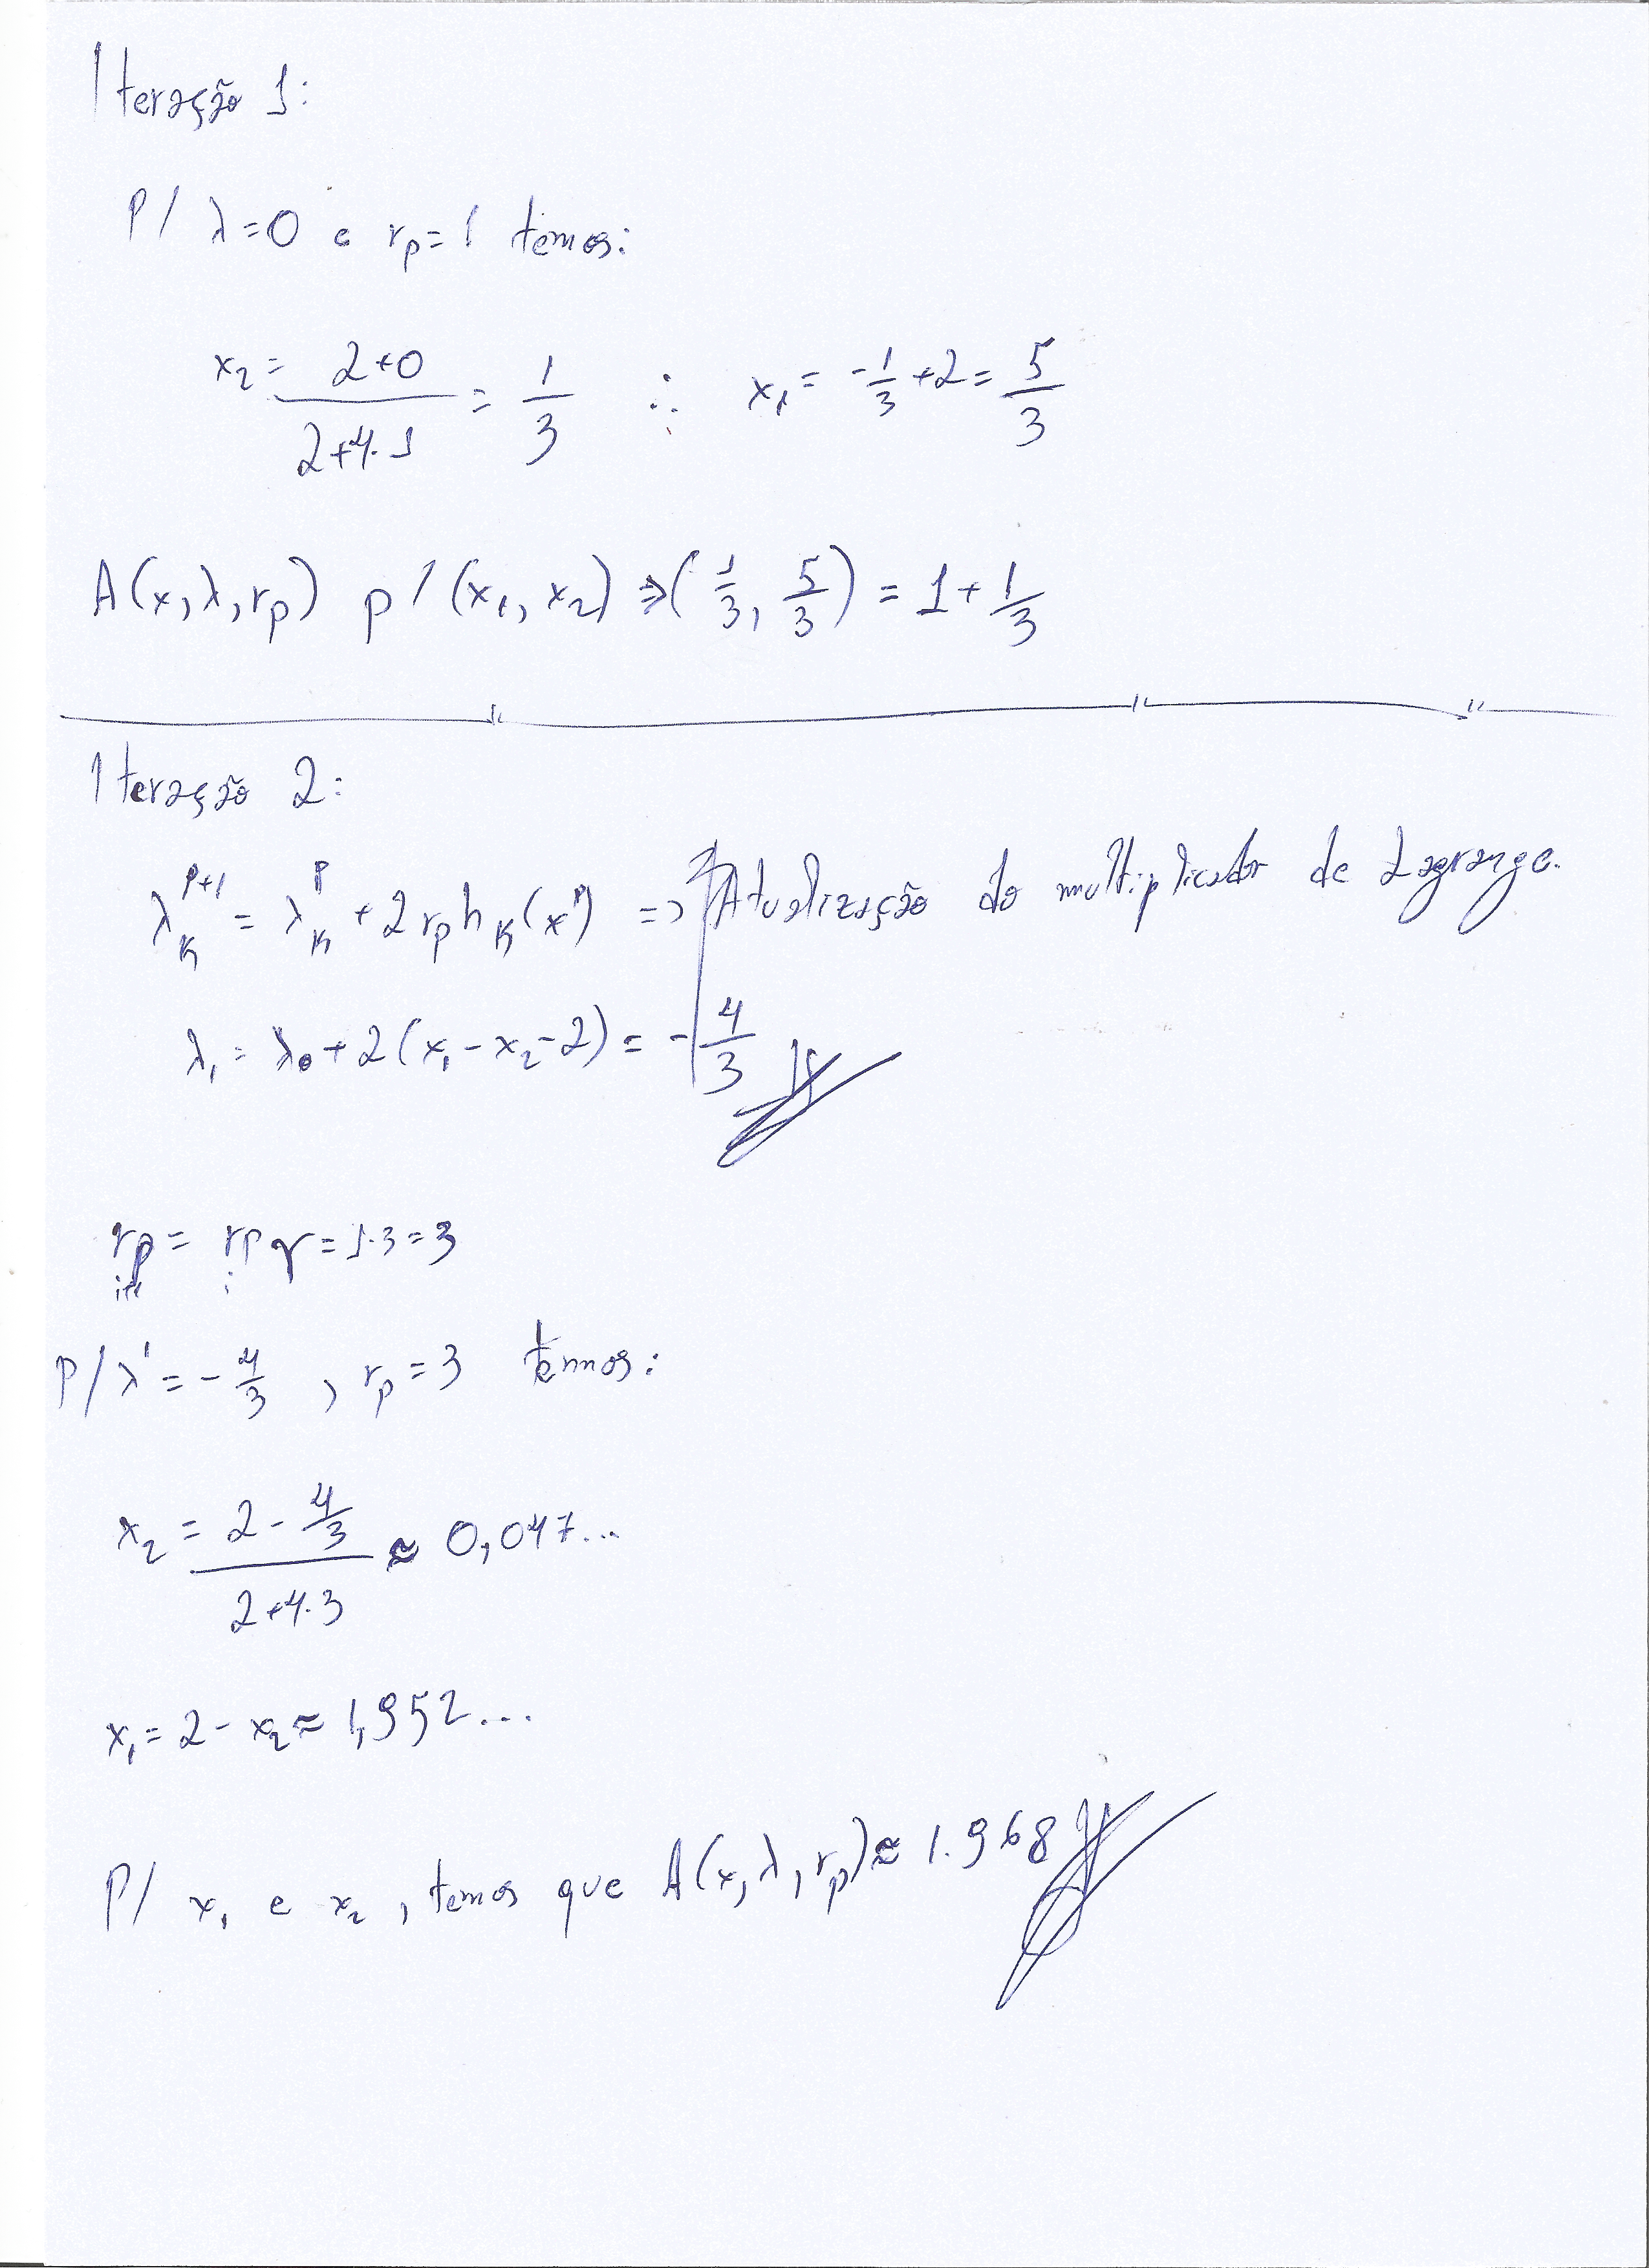
\includegraphics[width=\linewidth]{2_2.png}
\end{figure}%

\begin{figure}[H]
  \centering
  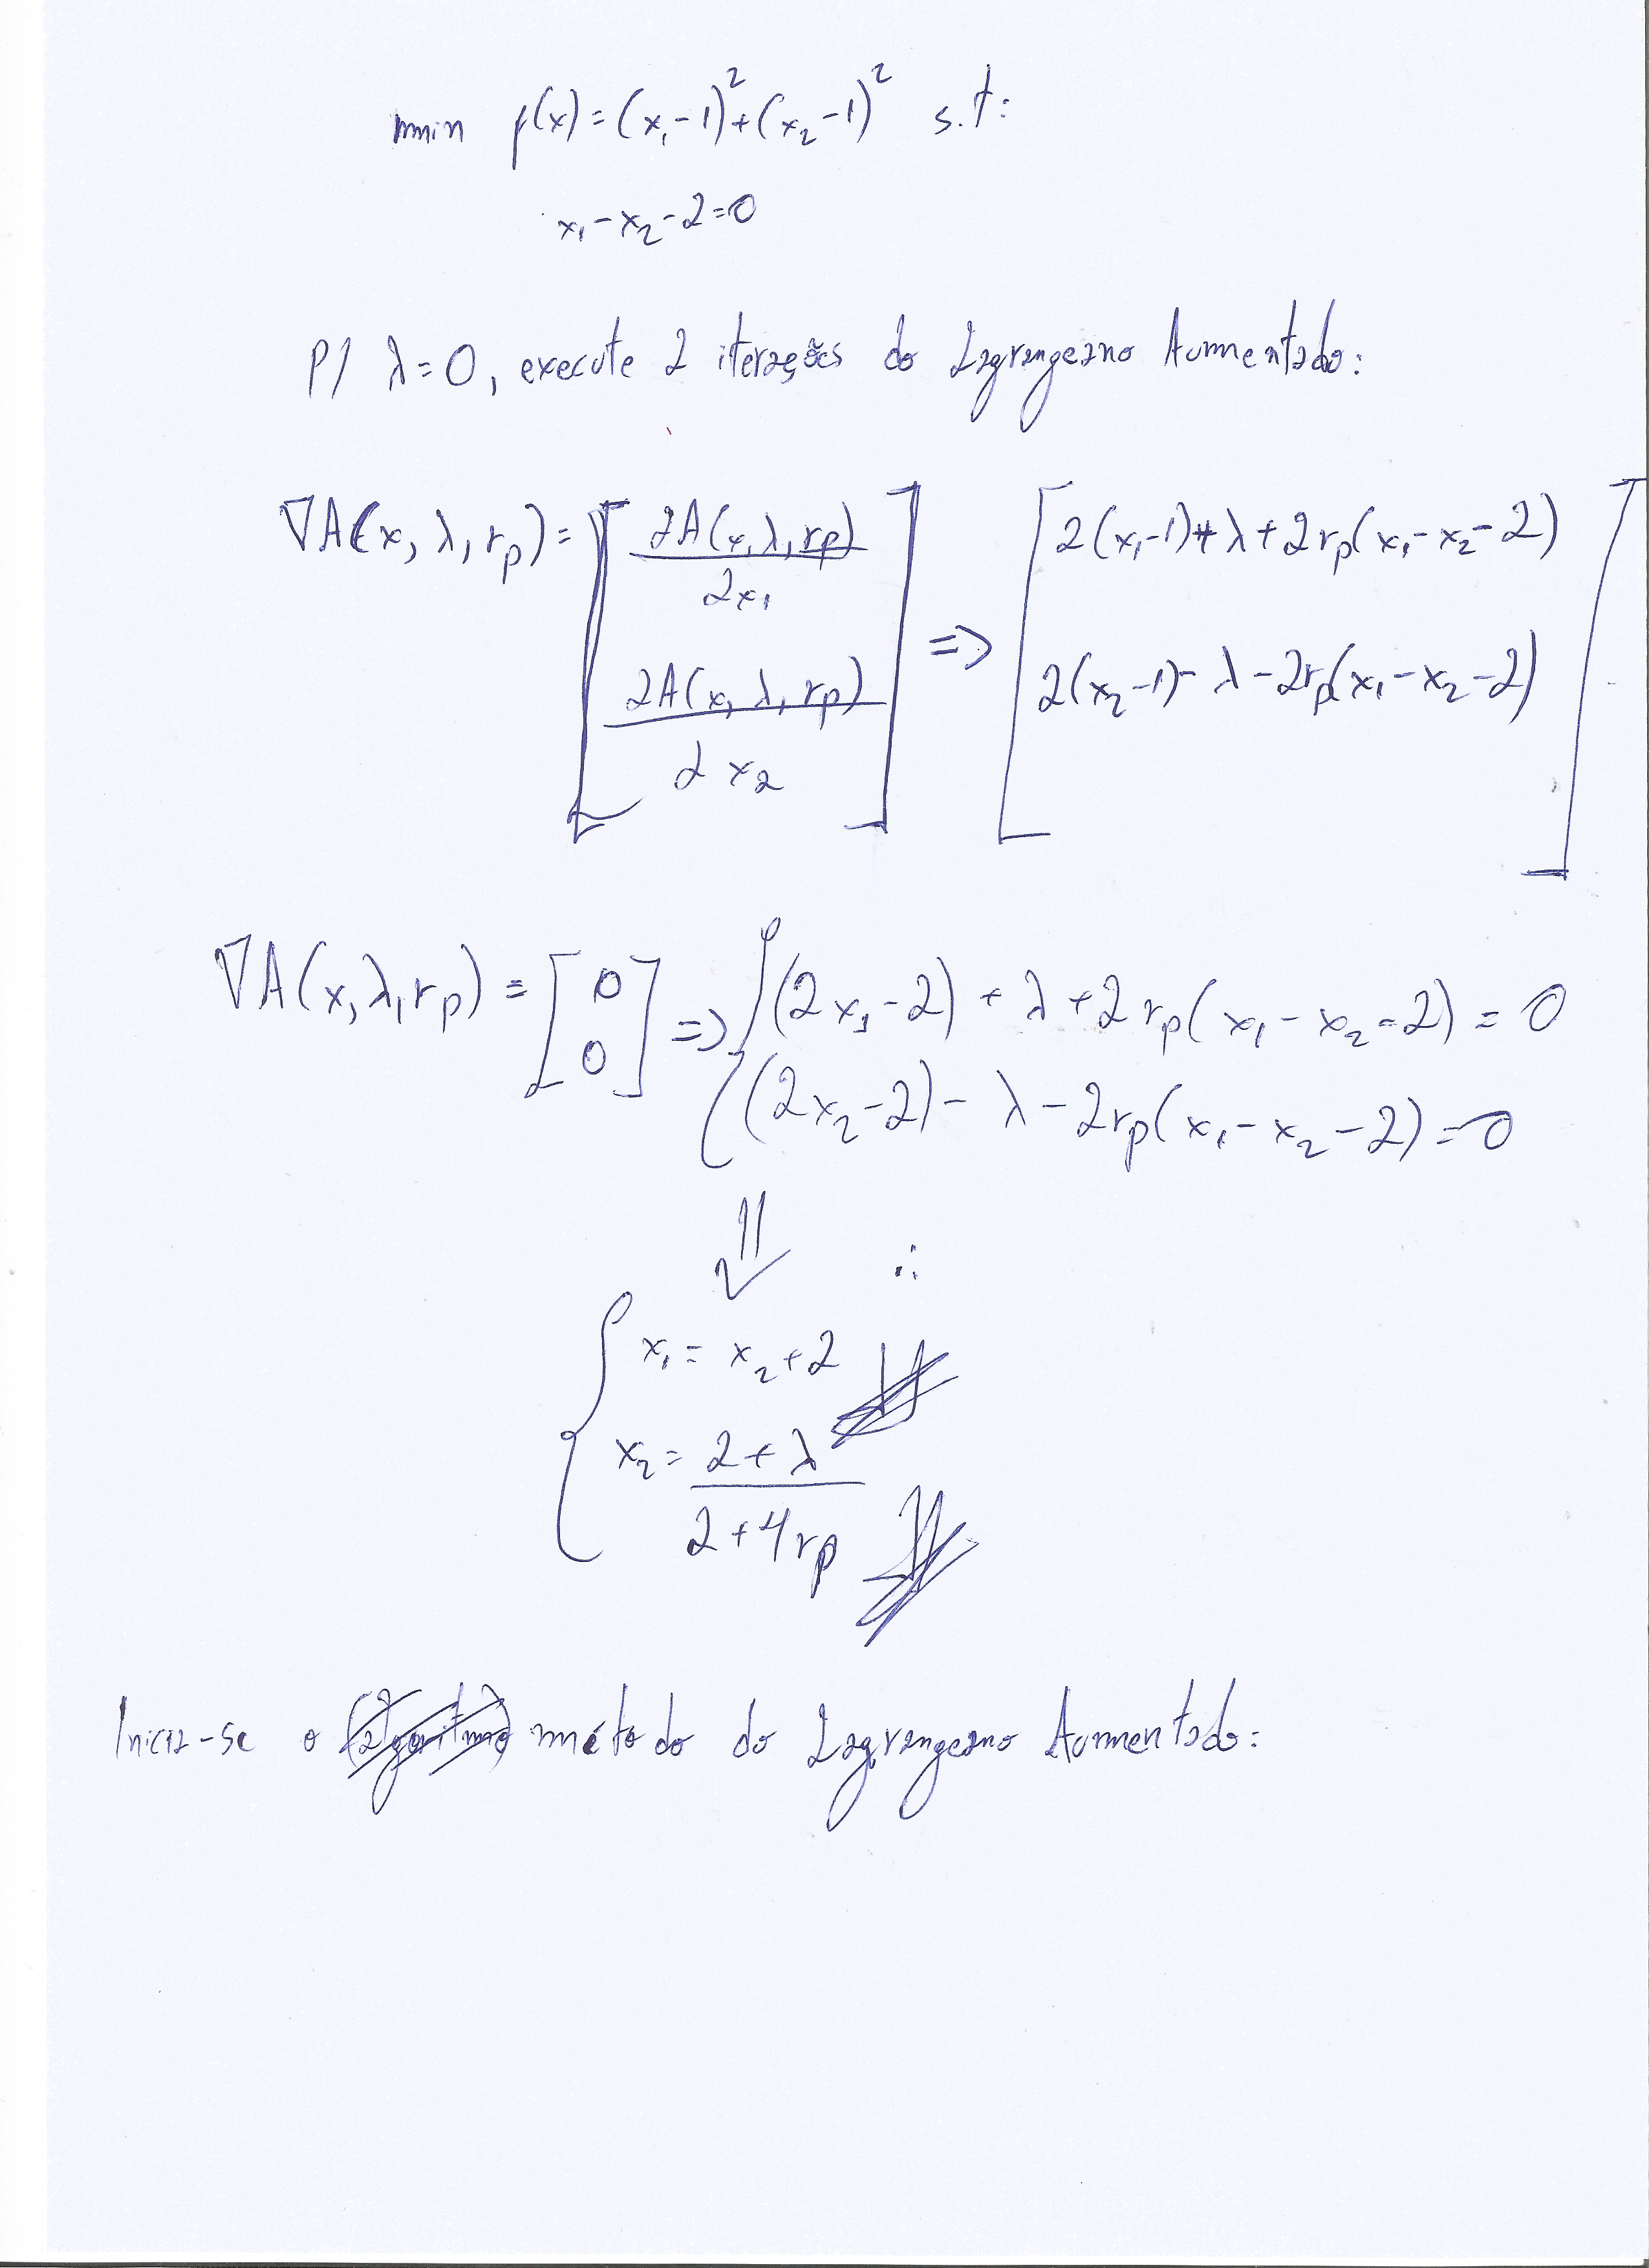
\includegraphics[width=\linewidth]{2_1.png}
\end{figure}%

\newpage
\section*{Questão 3}
\subsection*{Item A}
Considerando o seguinte problema de otimização:

\begin{align*}
\begin{split}
\text{min\phantom{0}} f(x_1,x_2) = (x_1 - 1)^2 + (x_2 - 1)^2 \text{\phantom{000} s.t:} \\
x_1 + x_2 - 0.5 \leq 0
\end{split}
\end{align*}

A função pseudo-objetivo na forma do Lagrangeano Aumentado é dada por:
\begin{align*}
\begin{split}
A (x,\lambda, r_P) = F(x) + \sum_{i=1}^{m} (\lambda_i \psi_i + r_P \psi_i^2)  \text{\phantom{000} tal que\phantom{0}} \psi_i \text{\phantom{0} é dado por:} \\
\psi_i = max \bigg (  g_i(x), \frac{- \lambda_i}{2 r_{P}} \bigg )
\end{split}
\end{align*}

Logo, tem-se:

\begin{align*}
\begin{split}
A(x,\lambda,r_P) = (x_1 - 1)^2 + (x_2 - 1)^2 + \lambda \bigg ( max \bigg( ( x_1+x_2-0.5),\frac{- \lambda}{2 r_{P}} \bigg) \bigg ) + \\
r_P \bigg ( max \bigg( (x_1 + x_2 - 0.5),\frac{- \lambda}{2 r_{P}} \bigg) \bigg ) ^2
\end{split}
\end{align*}

Visto que o chute inicial é $x = (1,1)$, temos que:

\begin{align*}
\begin{split}
\psi_i = max(g(1,1) = 1.5, 0) \\
\psi_i = x_1 + x_2 - 0.5 
\end{split}
\end{align*}

Logo, temos:

\begin{align*}
\begin{split}
A(x,\lambda, r_P) = (x_1 - 1)^2 + (x_2 - 1)^2 + \lambda (x_1 + x_2 - 0.5) + r_P (x_1 + x_2 - 0.5)^2
\end{split}
\end{align*}

Na forma de Penalidade Exterior, temos:

\begin{align*}
\begin{split}
\text{min\phantom{0}} f'(x) = F(x) + r_p P(x) \text{\phantom{000} tal que P(x) é dado por:} \\
P(x) = \sum_{i=1}^{n} (max(0,g_i(x)))^2 + \sum_{j=1}^{m} (h_k(x))^2 \\
f'(x) = (x_1 - 1)^2 + (x_2 - 1)^2 + r_p max (0,x_1 + x_2 - 0.5)^2
\end{split}
\end{align*}

Na forma de Penalidade Interior, temos:

\begin{align*}
\begin{split}
\text{min\phantom{0}} f'(x) = F(x) + r_p P(x) \text{\phantom{000} tal que P(x) é dado por:} \\
P(x) = \sum_{i=1}^{m} (\overline g_i(x)) +  \sum_{j=1}^{n} (h_j(x))^2 \\
\overline g_i(x) = 
\left\{\begin{matrix}
\frac{-1}{g_i(x)} \leftrightarrow g_i(x) \leq  \epsilon  \\ 
\frac{-2 \epsilon - g_i(x)}{\epsilon^2} | \epsilon = -C {r_P}^a, 
\end{matrix}\right.
\end{split}
\end{align*}

\newpage

\newpage
\section*{Questão 4}
\subsection*{Item A}
Considerando o seguinte problema de otimização:

\begin{align*}
\begin{split}
\text{min\phantom{0}} f(x_1,x_2) = (x_1 - 1)^2 + (x_2 - 1)^2 \text{\phantom{000} s.t:} \\
g(x) = x_1 + x_2 - 0.5 \leq 0 \\
h(x) = x_1 - x_2 - 2 = 0
\end{split}
\end{align*}

A função pseudo-objetivo na forma do Lagrangeano Aumentado é dada por:

\begin{align*}
\begin{split}
A(x,\lambda, r_P) = F(x) + \sum_{i=1}^{m} (\lambda_i \psi_i + r_P \psi_i^2) + \sum_{j=1}^{n} (\lambda_{j+m} h_j(x) + r_P (h_j(x))^2) \text{\phantom{0} tal que\phantom{0}} \psi_i \text{\phantom{0}é dado por:} \\
\end{split}
\end{align*}

\begin{align*}
\begin{split}
A(x,\lambda, r_P) = F(x) + \lambda_1 \bigg ( max \bigg ( g(x), \frac{- \lambda_1}{2 r_P} \bigg ) \bigg ) + \\
r_P \bigg ( max \bigg ( g(x), \frac{- \lambda_1}{2 r_P} \bigg ) \bigg )^2 + \\
\lambda_2 h(x) + r_P (h(x))^2
\end{split}
\end{align*}

\begin{align*}
\begin{split}
A(x,\lambda, r_P) = (x_1 - 1)^2 + (x_2 - 1)^2 + \lambda_1 (max \bigg ( \bigg (  (x_1 + x_2 - 0.5), \frac{- \lambda_1}{2 r_P} \bigg ) \bigg ) + \\
r_P \bigg ( max \bigg ( (x_1 + x_2 - 0.5, \frac{- \lambda_1}{2 r_P} \bigg ) \bigg )^2 + \\
\lambda_2 (x_1 - x_2 - 2) + r_P (x_1 - x_2 - 2)^2
\end{split}
\end{align*}

Considerando $x_1 = (1.0, 1.0)$, temos que:

\begin{align*}
\begin{split}
\psi = max(g(x) = 1.5, 0 ) = 1.5
\end{split}
\end{align*}


Logo, temos:

\begin{align*}
\begin{split}
A(x, \lambda, r_P) = (x_1 - 1)^2 + (x_2 - 1)^2 + \lambda_1 (x_1 + x_2 - 0.5) + \\ 
r_P (x_1 + x_2 - 0.5)^2 + \\
\lambda_2 (x_1 - x_2 - 2) + \\
r_P (x_1 - x_2 - 2)^2
\end{split}
\end{align*}

A função de penalidade exterior é dada por:

\begin{align*}
\begin{split}
\text{min\phantom{0}} f'(x) = F(x) + r_p P(x) \text{\phantom{000} tal que P(x) é dado por:} \\
P(x) = \sum_{i=1}^{n} (max(0,g_i(x)))^2 + \sum_{j=1}^{m} (h_k(x))^2 \\
f'(x) = (x_1-1)^2 + (x_2-1)^2 + r_p max (0,x_1 + x_2 - 0.5)^2 + (x_1 + x_2 - 0.5)^2
\end{split}
\end{align*}

\newpage
\section*{Questão 5}
\subsection*{Item A}
Foi realizada a minimização do problema de otimização abaixo utilizando os algoritmos de Newton, Powell, BFGS e Nelder-Mead através do Método da Penalidade Exterior:

\begin{align*}
\begin{split}
\text{min\phantom{0}} f(x_1,x_2) = x_1^2 + 2 x_2^2 - 2x_1 x_2 - 14x_1 - 14x_2 + 10 \text{\phantom{000} s.t:} \\
4x_1^2 + x_2^2 -25 \leq 0
\end{split}
\end{align*}

O $x*$ encontrado foi aproximadamente $(2.0, 3.0, -50)$ em todos os casos (com erro de $10^{-7}$). As figuras \ref{fig:Q5ABFGS},\ref{fig:Q5APowell} e \ref{fig:Q5ANelder-Mead} apresentam os $x*$ encontrados sob as curvas de nível e superfície da função, assim como a convergência dos algoritmos:

\begin{figure}[H]
\centering
\begin{subfigure}{0.3\textwidth}
  \centering
  \includegraphics[width=\linewidth]{5/MPFE/A/BFGS/contorno.png}
  %\caption{A subfigure}
\end{subfigure}%
\begin{subfigure}{0.3\textwidth}
  \centering
  \includegraphics[width=\linewidth]{5/MPFE/A/BFGS/superficie.png}
  %\caption{A subfigure}
\end{subfigure}
\begin{subfigure}{0.3\textwidth}
  \centering
  \includegraphics[width=\linewidth]{5/MPFE/A/BFGS/convergencia.png}
  %\caption{A subfigure}
\end{subfigure}
\caption{Curvas de nível, superfícies e séries de convergência para o algoritmo BFGS}
\label{fig:Q5ABFGS}
\end{figure}

\begin{figure}[H]
\centering
\begin{subfigure}{0.3\textwidth}
  \centering
  \includegraphics[width=\linewidth]{5/MPFE/A/Powell/contorno.png}
  %\caption{A subfigure}
\end{subfigure}%
\begin{subfigure}{0.3\textwidth}
  \centering
  \includegraphics[width=\linewidth]{5/MPFE/A/Powell/superficie.png}
  %\caption{A subfigure}
\end{subfigure}
\begin{subfigure}{0.3\textwidth}
  \centering
  \includegraphics[width=\linewidth]{5/MPFE/A/Powell/convergencia.png}
  %\caption{A subfigure}
\end{subfigure}
\caption{Curvas de nível, superfícies e séries de convergência para o algoritmo Powell}
\label{fig:Q5APowell}
\end{figure}

\begin{figure}[H]
\centering
\begin{subfigure}{0.3\textwidth}
  \centering
  \includegraphics[width=\linewidth]{5/MPFE/A/Nelder-Mead/contorno.png}
  %\caption{A subfigure}
\end{subfigure}%
\begin{subfigure}{0.3\textwidth}
  \centering
  \includegraphics[width=\linewidth]{5/MPFE/A/Nelder-Mead/superficie.png}
  %\caption{A subfigure}
\end{subfigure}
\begin{subfigure}{0.3\textwidth}
  \centering
  \includegraphics[width=\linewidth]{5/MPFE/A/Nelder-Mead/convergencia.png}
  %\caption{A subfigure}
\end{subfigure}
\caption{Curvas de nível, superfícies e séries de convergência para o algoritmo Nelder-Mead}
\label{fig:Q5ANelder-Mead}
\end{figure}


As tabelas abaixo apresentam a aproximação do $x*$ na execução de cada algoritmo:
\begin{longtable}[c]{|l|l|l|l|}
\hline
\multicolumn{1}{|c|}{x\_1} & \multicolumn{1}{c|}{x\_2} & \multicolumn{1}{c|}{f(x)} & \multicolumn{1}{c|}{erro} \\ \hline
\endfirsthead
%
\multicolumn{4}{c}%
{{\bfseries Continuação da Tabela \thetable\ da página anterior}} \\
\hline
\multicolumn{1}{|c|}{x\_1} & \multicolumn{1}{c|}{x\_2} & \multicolumn{1}{c|}{f(x)} & \multicolumn{1}{c|}{erro} \\ \hline
\endhead
%
1.8517490583488905         & 2.871413556211069         & -46.8395451048462         & 27.04908199658837         \\ \hline
1.9727000711264744         & 2.9766698644623175        & -49.42266027031416        & 2.1113216991046286        \\ \hline
1.9950082079576021         & 2.9957463378479234        & -49.89459071593174        & 0.3857671572697967        \\ \hline
1.9990864790334877         & 2.9992286401135075        & -49.980754890011006       & 0.07043291038843336       \\ \hline
1.9998228634367057         & 2.9998867425338536        & -49.996486253282626       & 0.012859319630159405      \\ \hline
1.9999542679482318         & 3.000015315516531         & -49.99936017630952        & 0.0023478521718658385     \\ \hline
1.9998532142484182         & 3.0003704977318097        & -49.999874009514784       & 0.0004258506799530437     \\ \hline
1.9998589495819121         & 3.0003726477472066        & -49.99997867704169        & 8.622756953258204e-05     \\ \hline
1.9998597436198093         & 3.000372945478484         & -49.99999316832337        & 1.2773734312077067e-05    \\ \hline
1.9998599631994842         & 3.0003730278184504        & -49.9999971757174         & 3.858705284187636e-06     \\ \hline
1.9998600692316302         & 3.000373067577115         & -49.99999911082206        & 1.8799086589638137e-06    \\ \hline
1.9998600707580148         & 3.0003730681837406        & -49.99999913888445        & 2.7818622072572907e-08    \\ \hline
\caption{Resolução do Item A via BFGS}
\label{tab:Q5A-BFGS}\\
\end{longtable}

% Please add the following required packages to your document preamble:
% \usepackage{longtable}
% Note: It may be necessary to compile the document several times to get a multi-page table to line up properly
\begin{longtable}[c]{|l|l|l|l|}
\hline
x\_1               & x\_2               & f(x)                & erro                   \\ \hline
\endfirsthead
%
\multicolumn{4}{c}%
{{\bfseries Continuação da Tabela \thetable\ da página anterior}} \\
\hline
x\_1               & x\_2               & f(x)                & erro                   \\ \hline
\endhead
%
1.8517490678563742 & 2.871413568446845  & -46.83954533342001  & 27.049081996588377     \\ \hline
1.9727001503527257 & 2.9766697013890835 & -49.42266055380941  & 2.111321478150053      \\ \hline
2.0020207774569747 & 2.977157893870329  & -49.89413987774088  & 0.3842109886290359     \\ \hline
2.0072932055405257 & 2.9772622376760323 & -49.97884584983822  & 0.06877348110932502    \\ \hline
2.00825314479338   & 2.9772819517983256 & -49.9942667029744   & 0.012511994606420274   \\ \hline
2.0084283232828763 & 2.977285554871725  & -49.99708068371458  & 0.0022828971404251774  \\ \hline
2.008460304562443  & 2.977286210056164  & -49.99759439291417  & 0.0004167475290230982  \\ \hline
2.008466143424055  & 2.9772863297131167 & -49.997688181462635 & 7.608614366461097e-05  \\ \hline
2.008467213494467  & 2.9772863406860433 & -49.99770530287921  & 1.3889409004264053e-05 \\ \hline
2.008467408861796  & 2.9772863426883056 & -49.99770842880238  & 2.535850278206908e-06  \\ \hline
2.0084674445324797 & 2.9772863430512944 & -49.997708999525884 & 4.629879839512796e-07  \\ \hline
\caption{Resolução do Item A via Powell}
\label{tab:Q5A-Powell}\\
\end{longtable}
\newpage

% Please add the following required packages to your document preamble:
% \usepackage{longtable}
% Note: It may be necessary to compile the document several times to get a multi-page table to line up properly
\begin{longtable}[c]{|l|l|l|l|}
\hline
x\_1               & x\_2               & f(x)                & erro                   \\ \hline
\endfirsthead
%
\multicolumn{4}{c}%
{{\bfseries Continuação da Tabela \thetable\ da página anterior}} \\
\hline
x\_1               & x\_2               & f(x)                & erro                   \\ \hline
\endhead
%
1.8517492001377192 & 2.871413566151038  & -46.83954744084904  & 27.049081996586743     \\ \hline
1.9727000439528872 & 2.9766697784253147 & -49.422659315767575 & 2.1113194409667386     \\ \hline
1.9950086383026266 & 2.9957452070132007 & -49.8945908091244   & 0.3857680800009078     \\ \hline
1.999088436843856  & 2.9992234174205725 & -49.98075487272487  & 0.07043282042396015    \\ \hline
1.999833430870394  & 2.9998585806293105 & -49.99648635707022  & 0.01285933996229005    \\ \hline
2.000157598726168  & 2.9994731410179933 & -49.999359679663904 & 0.0023466374543446022  \\ \hline
2.000216747330951  & 2.999402650649328  & -49.99988284161152  & 0.0004259534275732335  \\ \hline
2.0002275659553983 & 2.999389757331822  & -49.999978524957896 & 7.657035320107752e-05  \\ \hline
2.0002294075569558 & 2.9993875625886464 & -49.99999481266064  & 1.2724159233812316e-05 \\ \hline
2.0002297155372393 & 2.999387195551316  & -49.99999753653451  & 2.2263965746560643e-06 \\ \hline
2.0002298015765136 & 2.9993870930135285 & -49.999998297492695 & 2.1415040407646302e-07 \\ \hline
\caption{Resolução do Item A via Nelder-Mead}
\label{tab:Q5A-NelderMead}\\




\end{longtable}

\subsection*{Item B}
Foi realizada a minimização do problema de otimização abaixo utilizando os algoritmos de Newton, Powell, BFGS e Nelder-Mead através do Método da Penalidade Exterior:

\begin{align*}
\begin{split}
\text{min\phantom{0}} f(x) = x_1^2 + x_2^2 + 2 x_3^2 - x_4^2 - 5 x_1 - 5 x_2 - 21 x_3 + 7 x_4 + 100  \text{\phantom{000} s.t:} \\
x_1^2 + x_2^2 + x_3^2 + x_4^2 + x_1 - x_2 + x_3 - x_4 - 100 \\
x_1^2 + 2 x_2^2 + x_3^2 + 2 x_4^2 - x_1 - x_4 - 10 \\
2 x_1^2 + x_2^2 + x_3^2 + 2 x_1 - x_2 - x_4 - 5 \\
x_1-100 \leq 0 \\
x_2-100 \leq 0 \\
x_3-100 \leq 0 \\
x_4-100 \leq 0 \\
x_1+100 \leq 0 \\
x_2+100 \leq 0 \\
x_3+100 \leq 0 \\
x_4+100 \leq 0 \\
\end{split}
\end{align*}

O $x*$ encontrado foi aproximadamente $(-1.789, -1.400, -2.396, -1.6545, 168.598, 0.0)$ em todos os casos (com erro de $10^{-5}$). Não foi realizada a plotagem dos resultados obtidos devido a quantidade de variáveis da função.


A figura abaixo e as tabelas \ref{tab:Q5B-BFGS},\ref{tab:Q5B-Powell} e \ref{tab:Q5B-NelderMead} abaixo apresentam a aproximação do $x*$ na execução de cada algoritmo:


\begin{figure}[H]
\centering
\begin{subfigure}{0.3\textwidth}
  \centering
  \includegraphics[width=\linewidth]{5/MPFE/B/BFGS/convergencia.png}
  \caption{Convergência do algoritmo BFGS}
\end{subfigure}%
\begin{subfigure}{0.3\textwidth}
  \centering
  \includegraphics[width=\linewidth]{5/MPFE/A/Powell/convergencia.png}
  \caption{Convergência do algoritmo Powell}
\end{subfigure}
\begin{subfigure}{0.3\textwidth}
  \centering
  \includegraphics[width=\linewidth]{5/MPFE/A/Nelder-Mead/convergencia.png}
  \caption{Convergência do algoritmo Nelder-Mead}
\end{subfigure}
\label{fig:Q5BConvergencia}
\end{figure}


% Please add the following required packages to your document preamble:
% \usepackage{longtable}
% Note: It may be necessary to compile the document several times to get a multi-page table to line up properly
\begin{longtable}[c]{|l|l|l|l|l|l|}
\hline
\multicolumn{1}{|c|}{x\_1} & \multicolumn{1}{c|}{x\_2} & \multicolumn{1}{c|}{x\_3} & \multicolumn{1}{c|}{x\_4} & \multicolumn{1}{c|}{f(x)} & \multicolumn{1}{c|}{erro} \\ \hline
\endfirsthead
%
\multicolumn{6}{c}%
{{\bfseries Continuação da Tabela \thetable\ da página anterior}} \\
\hline
\multicolumn{1}{|c|}{x\_1} & \multicolumn{1}{c|}{x\_2} & \multicolumn{1}{c|}{x\_3} & \multicolumn{1}{c|}{x\_4} & \multicolumn{1}{c|}{f(x)} & \multicolumn{1}{c|}{erro} \\ \hline
\endhead
%
-1,79095                   & -1,40019                  & -2,37144                  & -1,66819                  & 167,71121                 & 12150,99165               \\ \hline
-1,78987                   & -1,40011                  & -2,38806                  & -1,65907                  & 168,30295                 & 0,59176                   \\ \hline
-1,78951                   & -1,40007                  & -2,39359                  & -1,65602                  & 168,49982                 & 0,19678                   \\ \hline
-1,78939                   & -1,40006                  & -2,39543                  & -1,65501                  & 168,56550                 & 0,06571                   \\ \hline
-1,78935                   & -1,40005                  & -2,39605                  & -1,65467                  & 168,58740                 & 0,02189                   \\ \hline
-1,78934                   & -1,40005                  & -2,39625                  & -1,65456                  & 168,59478                 & 0,00726                   \\ \hline
-1,78934                   & -1,40005                  & -2,39632                  & -1,65452                  & 168,59702                 & 0,00223                   \\ \hline
-1,78933                   & -1,40005                  & -2,39634                  & -1,65451                  & 168,59792                 & 0,00101                   \\ \hline
-1,78933                   & -1,40005                  & -2,39635                  & -1,65451                  & 168,59818                 & 0,00017                   \\ \hline
-1,78933                   & -1,40005                  & -2,39635                  & -1,65451                  & 168,59818                 & 0,00000                   \\ \hline
\caption{Minimização via BFGS}
\label{tab:Q5B-BFGS}\\
\end{longtable}

% Please add the following required packages to your document preamble:
% \usepackage{longtable}
% Note: It may be necessary to compile the document several times to get a multi-page table to line up properly
\begin{longtable}[c]{|l|l|l|l|l|l|}
\hline
\multicolumn{1}{|c|}{x\_1} & \multicolumn{1}{c|}{x\_2} & \multicolumn{1}{c|}{x\_3} & \multicolumn{1}{c|}{x\_4} & \multicolumn{1}{c|}{f(x)} & \multicolumn{1}{c|}{erro} \\ \hline
\endfirsthead
%
\multicolumn{6}{c}%
{{\bfseries Continuação da Tabela \thetable\ da página anterior}} \\
\hline
\multicolumn{1}{|c|}{x\_1} & \multicolumn{1}{c|}{x\_2} & \multicolumn{1}{c|}{x\_3} & \multicolumn{1}{c|}{x\_4} & \multicolumn{1}{c|}{f(x)} & \multicolumn{1}{c|}{erro} \\ \hline
\endhead
%
-1,79227                   & -1,39709                  & -2,37280                  & -1,66723                  & 167,74989                 & 12150,98167               \\ \hline
-1,79473                   & -1,40085                  & -2,38124                  & -1,65955                  & 168,13687                 & 0,44239                   \\ \hline
-1,79326                   & -1,40206                  & -2,38891                  & -1,65556                  & 168,40925                 & 0,65220                   \\ \hline
-1,79119                   & -1,40174                  & -2,39335                  & -1,65441                  & 168,53661                 & 0,63089                   \\ \hline
-1,78991                   & -1,40102                  & -2,39537                  & -1,65430                  & 168,58294                 & 0,47526                   \\ \hline
-1,78941                   & -1,40049                  & -2,39611                  & -1,65440                  & 168,59607                 & 0,26315                   \\ \hline
-1,78929                   & -1,40021                  & -2,39632                  & -1,65447                  & 168,59856                 & 0,10846                   \\ \hline
-1,78929                   & -1,40009                  & -2,39636                  & -1,65450                  & 168,59858                 & 0,03668                   \\ \hline
-1,78931                   & -1,40006                  & -2,39636                  & -1,65450                  & 168,59837                 & 0,01305                   \\ \hline
-1,78932                   & -1,40005                  & -2,39636                  & -1,65450                  & 168,59829                 & 0,00549                   \\ \hline
-1,78933                   & -1,40005                  & -2,39635                  & -1,65450                  & 168,59829                 & 0,00245                   \\ \hline
-1,78933                   & -1,40005                  & -2,39635                  & -1,65450                  & 168,59830                 & 0,00078                   \\ \hline
-1,78933                   & -1,40005                  & -2,39635                  & -1,65450                  & 168,59832                 & 0,00021                   \\ \hline
-1,78933                   & -1,40005                  & -2,39635                  & -1,65450                  & 168,59832                 & 0,00000                   \\ \hline
\caption{Minimização via Powell}
\label{tab:Q5B-Powell}\\
\end{longtable}
% Please add the following required packages to your document preamble:
% \usepackage{longtable}
% Note: It may be necessary to compile the document several times to get a multi-page table to line up properly
\begin{longtable}[c]{|l|l|l|l|l|l|}
\hline
x\_1     & x\_2     & x\_3     & x\_4     & f(x)      & erro        \\ \hline
\endfirsthead
%
\multicolumn{6}{c}%
{{\bfseries Continuação da Tabela \thetable\ da página anterior}} \\
\hline
x\_1     & x\_2     & x\_3     & x\_4     & f(x)      & erro        \\ \hline
\endhead
%
-1,79095 & -1,40019 & -2,37144 & -1,66819 & 167,71130 & 12150,99165 \\ \hline
-1,78987 & -1,40010 & -2,38806 & -1,65907 & 168,30282 & 0,59159     \\ \hline
-1,78951 & -1,40007 & -2,39359 & -1,65602 & 168,49985 & 0,19703     \\ \hline
-1,78939 & -1,40006 & -2,39543 & -1,65501 & 168,56550 & 0,06565     \\ \hline
-1,78935 & -1,40005 & -2,39605 & -1,65467 & 168,58737 & 0,02188     \\ \hline
-1,78934 & -1,40005 & -2,39625 & -1,65456 & 168,59466 & 0,00731     \\ \hline
-1,78933 & -1,40005 & -2,39632 & -1,65452 & 168,59713 & 0,00247     \\ \hline
-1,78933 & -1,40005 & -2,39634 & -1,65451 & 168,59792 & 0,00078     \\ \hline
-1,78933 & -1,40005 & -2,39635 & -1,65450 & 168,59818 & 0,00027     \\ \hline
-1,78933 & -1,40005 & -2,39635 & -1,65450 & 168,59829 & 0,00010     \\ \hline
-1,78933 & -1,40005 & -2,39635 & -1,65450 & 168,59831 & 0,00002     \\ \hline
-1,78933 & -1,40005 & -2,39635 & -1,65450 & 168,59831 & 0,00000     \\ \hline
\caption{Minimização via Nelder-Mead}
\label{tab:Q5B-NelderMead}\\
\end{longtable}

\newpage
\section*{Questão 6}
Considerando o problema de otimização abaixo:
\begin{figure}[H]
  \centering
  \includegraphics[width=0.3\linewidth]{6/trelica.png}
  \caption{Treliça de 4 barras}
\end{figure}
\begin{align*}
\begin{split}
\text{max\phantom{0}} f(x_1,x_2) = (9 - (x_1 -3)^2) \frac{x_2^3}{27 \sqrt{3}} \text{\phantom{000} s.t:} \\ 
x_1 \geq 0 \\
0 \leq x_2 \leq \frac{x_1}{\sqrt{3}} \\
0 \leq  x_1 + \sqrt{3}x_2  \leq 6
\end{split}
\end{align*}

Este foi resolvido utilizando 2 métodos de otimização irrestrita (BFGS e Nelder-Mead) através do Método da Penalidade Exterior, para tanto, o problema inicial foi reescrito da seguinte forma:

\begin{align*}
\begin{split}
\text{min\phantom{0}} f(x_1,x_2) = (-1)  \bigg( (9-(x_1-3)^2)  \bigg( \frac{x_1^3}{27 \sqrt{3}} \bigg ) \bigg )  \text{\phantom{000} s.t:}\\
x_1+ \sqrt{3} x_2-6  \leq 0\\
x_2 - \frac{x_1}{\sqrt{3}} \leq 0 \\
-x_1  \leq 0\\
\end{split}
\end{align*}

E finalmente:

\begin{align*}
\begin{split}
\text{min\phantom{0}} f'(x_1,x_2) = (-1)  \bigg( (9-(x_1-3)^2)  \bigg( \frac{x_1^3}{27 \sqrt{3}} \bigg ) \bigg ) + r_P \bigg ( (x_1+ \sqrt{3}*x_2-6)^2 + \bigg (x_2 - \frac{x_1}{\sqrt{3}} \bigg )^2 \bigg )
\end{split}
\end{align*}

Foi encontrado um $x*$ ótimo igual a $(3, \sqrt{3},-1)$ no algoritmo de Nelder-Mead, e o mesmo resultado (com erro da ordem de $10^{-7}$) no algoritmo BFGS, ambos com 7 iterações. É sabido que existe outro $x*$  desta função, $(0.000183308, -0.156902, 0.0)$, entretanto nenhum dos experimentos elaborados foi capaz de retornar tal $x*$.
As figuras \ref{fig:Q6NelderMead} e \ref{fig:Q6BFGS} apresentam o mínimo da função sob as curvas de nível e superfície das mesmas, assim como a convergência de cada algoritmo durante a execução do problema descrito:

\begin{figure}[H]
\centering
\begin{subfigure}{0.3\textwidth}
  \centering
  \includegraphics[width=\linewidth]{6/Nelder-Mead/contorno.png}
  %\caption{A subfigure}
\end{subfigure}%
\begin{subfigure}{0.3\textwidth}
  \centering
  \includegraphics[width=\linewidth]{6/Nelder-Mead/superficie.png}
  %\caption{A subfigure}
\end{subfigure}
\begin{subfigure}{0.3\textwidth}
  \centering
  \includegraphics[width=\linewidth]{6/Nelder-Mead/convergencia.png}
  %\caption{A subfigure}
\end{subfigure}
\caption{Curvas de nível, superfícies e séries de convergência para o algoritmo Nelder-Mead}
\label{fig:Q6NelderMead}
\end{figure}

\begin{figure}[H]
\centering
\begin{subfigure}{0.3\textwidth}
  \centering
  \includegraphics[width=\linewidth]{6/BFGS/contorno.png}
  %\caption{A subfigure}
\end{subfigure}%
\begin{subfigure}{0.3\textwidth}
  \centering
  \includegraphics[width=\linewidth]{6/BFGS/superficie.png}
  %\caption{A subfigure}
\end{subfigure}
\begin{subfigure}{0.3\textwidth}
  \centering
  \includegraphics[width=\linewidth]{6/BFGS/convergencia.png}
  %\caption{A subfigure}
\end{subfigure}
\caption{Curvas de nível, superfícies e séries de convergência para o algoritmo BFGS}
\label{fig:Q6BFGS}
\end{figure}

Os dados apresentados acima foram gerados à partir das tabelas abaixo:

\begin{longtable}[c]{|l|l|l|l|}
\hline
\multicolumn{1}{|c|}{x\_1} & \multicolumn{1}{c|}{x\_2} & \multicolumn{1}{c|}{f(x)} & \multicolumn{1}{c|}{erro} \\ \hline
\endfirsthead
%
\multicolumn{4}{c}%
{{\bfseries Continuação da Tabela \thetable\ da página anterior}} \\
\hline
\multicolumn{1}{|c|}{x\_1} & \multicolumn{1}{c|}{x\_2} & \multicolumn{1}{c|}{f(x)} & \multicolumn{1}{c|}{erro} \\ \hline
\endhead
%
2.9999747780098738         & 1.7320795641239406        & -1.0000498085706777       & 1787.2210578233385        \\ \hline
2.9999868106124943         & 1.7320609013961183        & -1.0000174831041808       & 3.214210625512859e-05     \\ \hline
2.9999917236288516         & 1.732053282069772         & -1.0000042859597853       & 1.1951566638690458e-05    \\ \hline
2.9999941624392235         & 1.7320494998353593        & -0.9999977349370279       & 6.5034268849073484e-06    \\ \hline
2.9999949358875937         & 1.7320483003352463        & -0.9999956573474016       & 1.2278195206105735e-06    \\ \hline
2.9999949358875937         & 1.7320483003352463        & -0.9999956573474016       & 0.0                       \\ \hline
\caption{Resolução do problema de otimização via Nelder-Mead}
\label{tab:Q6-NelderMead}\\
\end{longtable}

% Please add the following required packages to your document preamble:
% \usepackage{longtable}
% Note: It may be necessary to compile the document several times to get a multi-page table to line up properly
\begin{longtable}[c]{|l|l|l|l|}
\hline
\multicolumn{1}{|c|}{x\_1} & \multicolumn{1}{c|}{x\_2} & \multicolumn{1}{c|}{f(x)} & \multicolumn{1}{c|}{erro} \\ \hline
\endfirsthead
%
\multicolumn{4}{c}%
{{\bfseries Continuação da Tabela \thetable\ da página anterior}} \\
\hline
\multicolumn{1}{|c|}{x\_1} & \multicolumn{1}{c|}{x\_2} & \multicolumn{1}{c|}{f(x)} & \multicolumn{1}{c|}{erro} \\ \hline
\endhead
%
2.9999749981166355         & 1.732079668896944         & -1.000049990050108        & 1787.2210578250624        \\ \hline
2.999991666937979          & 1.7320604240912012        & -1.0000166563900192       & 3.331122909755457e-05     \\ \hline
2.9999972208843695         & 1.7320540080148927        & -1.0000055433444905       & 1.1090305371164177e-05    \\ \hline
2.999999072742912          & 1.7320518696720812        & -1.0000018396177448       & 3.6792543515185017e-06    \\ \hline
2.999999690610147          & 1.7320511572355557        & -1.0000006056405644       & 1.2101214538207117e-06    \\ \hline
2.9999998957883656         & 1.7320509192988323        & -1.0000001935219702       & 3.881609342837322e-07     \\ \hline
\caption{}
\label{tab:Q6-BFGS}\\
\end{longtable}

O problema também foi resolvido através dos algoritmos SLSQP (Sequential Least Squares Programming) e Cobyla (Constraints by Linear Approximations), visto que ambos os métodos foram capazes de atingir os resultados apresentados anteriormente, as plotagens dos gráficos foram emitidas. Notou-se que o SLSQP levou 5 iterações, 20 avaliações da função objetivo e 5 avaliações do gradiente para convergir até um resultado aceitável, enquanto que o algoritmo Cobyla levou 14 iterações, e 26 avaliações da função objetivo para atingir um resultado dentro da margem de tolerância padrão ($10^{-6}$).


\begin{longtable}[c]{|l|l|l|}
\hline
\multicolumn{1}{|c|}{x\_1} & \multicolumn{1}{c|}{x\_2} & \multicolumn{1}{c|}{f(x)} \\ \hline
\endfirsthead
%


\multicolumn{3}{c}%
{{\bfseries Table \thetable\ continued from previous page}} \\
\hline
\multicolumn{1}{|c|}{x\_1} & \multicolumn{1}{c|}{x\_2} & \multicolumn{1}{c|}{f(x)} \\ \hline
\endhead
%
1.3860516216884882         & 0.80023727576844728       & -0.070078383768581873     \\ \hline
1.5306770535297327         & 0.88373680847664904       & -0.10096474433628834      \\ \hline
2.4633471432328333         & 1.4222141404861244        & -0.53590602198628878      \\ \hline
3.0000000096336938         & 1.7320508075702321        & -1.0000000000023468       \\ \hline
3.0000000096336938         & 1.7320508075702321        & -1.0000000000023468       \\ \hline
\caption{Resolução do problema de otimização via SQP}
\label{tab:SQP}\\
\end{longtable}

Um resultado semelhante foi apresentado pelo Método Cobyla (Constrained optimization by linear approximation), podendo ser encontrado nos arquivos em anexo (no arquivo cobyla.py).


\end{document}


%\begin{align*}
%\begin{split}
%H(f(x)) =
%\begin{bmatrix}
%\frac{16 \pi x_2 ^{2}}{(3x_1 ^{2}+10x_1 x_2 +3x_2 ^{2})^{\frac{3}{2}}} & -\frac{16 \pi x_1  x_2 }{(3 x_1 ^2 + 10 x_1  %x_2  + 3 x_2 ^2)^{3/2}} \\
%-\frac{16 \pi x_1  x_2 }{(3 x_1 ^2 + 10 x_1  x_2  + 3 x_2 ^2)^{3/2}} & \frac{16 \pi x_1 ^{2}}{(3x_1 ^{2}+10x_1 x_2 %+3x_2 ^{2})^{\frac{3}{2}}}
%\end{bmatrix}
%\end{split}
%\end{align*}


%\begin{figure}[H]
%\label{figure:fig1}
%   \center{\includegraphics[width=\textwidth]{2_contorno.png}}
%   \caption{Curvas de nível e superfície da função, assim como o vetor de descida máxima}
%\end{figure}
